
% Currently supported format is the old 4:3 aspect ratio (and not for 16:9)
% You need to select the LuaTeX engine to compile to pdf, perhaps XeTeX would also work
% If you use Overleaf, you have to change the compiler (https://www.overleaf.com/learn/how-to/Changing_compiler)
% Reason: The common pdfTeX engine cannot use system fonts: Calibri, Georgia
% LuaTeX needs a little bit longer to compile

\documentclass[aspectratio=43]{beamer}

% Load package "amsmath" before PSI43 (because "fontspec" inside PSI43 should be loaded before)
% For other packages, it seems not to matter
\usepackage{amsmath}

% Because of LuaTeX, packages "fontenc", "inputenc", "textcomp" should not be loaded

\usepackage{PSI43} % "PSI43" has no side effects, apart from loading package "fontspec"


% Change the following colors to your liking (if commented out -> no colors):
\setbeamercolor{block body alerted}{bg=alerted text.fg!10}
\setbeamercolor{block title alerted}{bg=alerted text.fg!20}
\setbeamercolor{block body}{bg=structure!10}
\setbeamercolor{block title}{bg=structure!20}
\setbeamercolor{block body example}{bg=green!10}
\setbeamercolor{block title example}{bg=green!20}





\begin{document}

\title{A novel approach to energy system analysis and technology assessment}
\author{Ludwig Wittgenstein}
\institute{Laboratory of Energy Systems Analysis, Paul Scherrer Institute}
\PSIsubtitle{Line 1\\Line 2 (a 3rd line may be required for single-line titles to move gray box down)}


\begin{frame}[plain] % plain prohibits logo, footer etc.
  \titlepage
\end{frame}


\begin{frame}{A list that is reveiled}  
  \begin{itemize}
  \item<1-> Item 1
  \item[-]<1->  Item 1 (with dash as bullet)
    \begin{itemize}
    \item<1-> Item 1b
    \end{itemize}
  \item<2->  Item 2 (revealed on next slide)
  \item<3-> Item 3
    \begin{itemize}
    \item<3-> Item 4
      \begin{itemize}
      \item<3-> Item 5
      \end{itemize}
    \end{itemize}
  \end{itemize}
 \vspace*{\fill} % to put the text a little bit upwards
\end{frame}



\begin{frame}[squeeze]{Titles over two lines are possible 11111 11111 1111 1111  11111 11111 1111  11111 111  1111 1111}
  \alert{This is a frame with the usual `squeeze' option of beamer to narrow linespacing a little bit, The color of this text is called ``alert'' in beamer}
  
  \structure{This is a color predefined in beamer called ``structure''}
  \begin{align*}
    a + b  & = \int_a^b f(x)\,dx \\
    \sum_{n=1}^N x_{i_n} &= \frac{a+b}{c+d} 
  \end{align*}
  \begin{itemize}
  \item  $\alpha = \zeta$ 
  \item $\mathcal{F}_t$, $\mathbb{R}^n$
  \item $\{t \mid t=1,\dots,T\}$
  \item $f\colon x\to y$
  \end{itemize}  
\end{frame}

\begin{frame}{Columns and Blocks}
  You can start text very high with the space command with the code in the  .tex file of this slide

  The color of the blocks are defined in the preamble of the .tex file:
  \begin{columns}
    \begin{column}[T]{4cm}
      \centering
      \begin{block}{Text in a block}
        This is a block of text in the first column
      \end{block}
      \begin{exampleblock}{Text in a example block}
        This is a block of text in the first column
      \end{exampleblock}
      Text outside of block in first column
    \end{column}
    \begin{column}[T]{4cm}
      \begin{block}{Text in a block}
        This is a block 
      \end{block}
      \begin{alertblock}{Text in an alert block}
        This is a block
      \end{alertblock}
    \end{column}
  \end{columns}
    
    \vskip 0pt plus 1filll
 \end{frame}


 \begin{frame}{Text}
   \vspace*{3.7ex}
  You can start text a little bit lower with the command in this slide
  \begin{figure}
    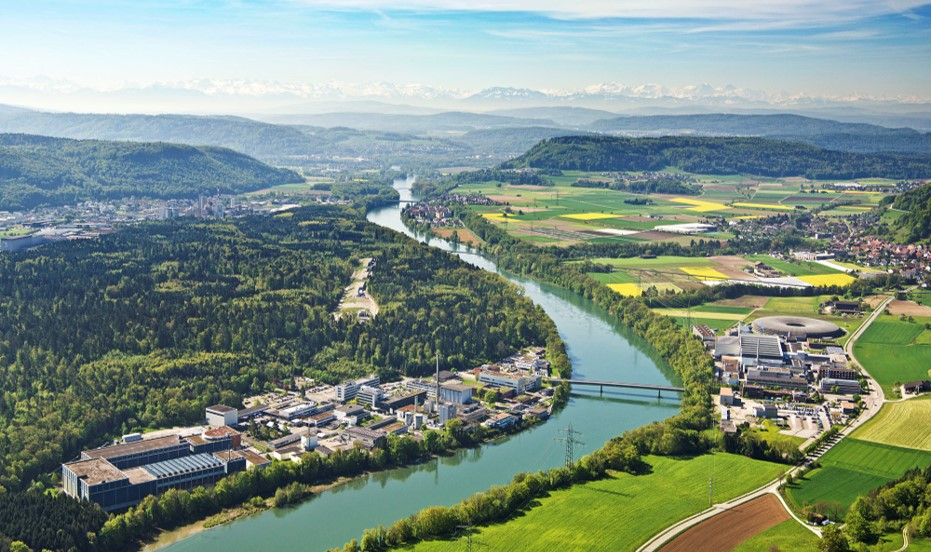
\includegraphics[width=0.3\pagewidth]{PSIlandscape}
    \caption{Figures are automatically centered}
    \label{fig:PSI}
    \end{figure}

     \vskip 0pt plus 1filll
\end{frame}

\PSItrailer{
    \textbf{My thanks go to}
     \smallskip
    \begin{itemize}
    \item Co-author 1
    \item Co-author with verrry loong name 2
    \item Supervisor 1
    \item Supervisor 2  
    \end{itemize}
    }
  

\end{document}

% The following can be deleted if not the EMACS editor is used for editing

%%%Local Variables:
%%% mode: latex
%%% TeX-master: t
%%% TeX-engine: luatex
%%% End:
